

\subsection{Parallelize rectilinear lossless wavelet transform}
\subsubsection{Single core CPU implementation}
We attempt to implement a single core CPU version of 2D DWT to have a ground truth for performance comparison with other famous libraries we mentioned above and our next parallel version on the GPU.

Firstly, let us explain the insight of lifting scheme version of 2 types of biorthogonal wavelet families we will deal with: Haar and CDF5/3~\cite{daubechies1992ten}.

\subsubsection{Multi core GPU implementation with filter scheme}
\subsubsection{Multi core GPU implementation with lifting scheme}


%%
\subsection{Perform a one-step self-localization of wavelet coefficients in mixed-band wavelet domain}
\label{subsec:onestepfilter}
The noisy image is firstly transformed to a wavelet domain using lossless biorthogonal wavelet families such as Haar or CDF5/3~\cite{daubechies1992ten}
\subsubsection{Using a mean filter}
\subsubsection{Using a median filter}
\subsubsection{Using a Gaussian filter}
\subsubsection{Using a bilateral filter}

% \subsection{Extend to 3D MRI denoising}
% 3D images acquired from an MRI scanner also contain noise-like impacts (see Fig.~\ref{fig:3dmri}) which come from the high-damped vibrations of signals due to the affects from electro-magnetic waves to water molecules. 
% To reduce such that effects, people employ the smoothing metrics by introducing total variation regularizers into an energy function that they attempt to minimize and iteratively threshold the intermediate results.
% \begin{figure}[t]
	% \centering  
	%%%%%%%%%%%%%%%%%%%%%%%%%%%%%%%%%%%%%%%%%%%%%%%%%%%%%%%%%%%%%%%%%%%%%%
	% \subfloat[]
    % {  
  		% 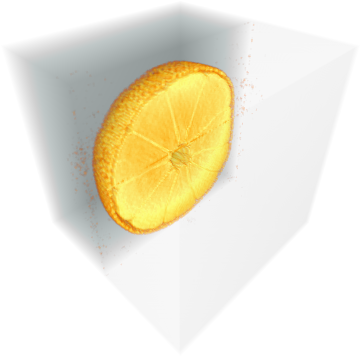
\includegraphics[width=0.5\linewidth]{fig/tangerine128_crop.png}
	% }	
    % \subfloat[]
    % {
		% 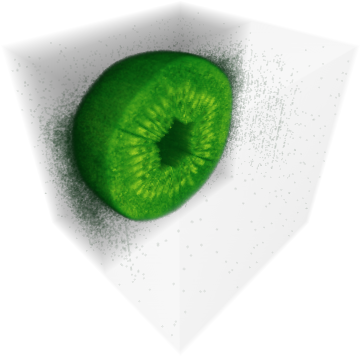
\includegraphics[width=0.5\linewidth]{fig/kiwi128_crop.png}
    % }	
% \caption{TODO}
% \label{fig:3dmri}
% \end{figure}

\subsection{Extend to 3D CSMRI Reconstruction}
In brief, the data come from MRI modality is so-called k-space which represents the samples of the spectrum of the images. 
To get the actual images we want to look at, an inverse Fourier transform is necessary to apply. 
Usually, the scanning procedure requires a long period to obtain the k-space and sometimes cause the danger to such an emergency situation. 
One way to circumvent this case is to discard randomly most of the k-space. 
But if we do not introduce some constraints (e.g, images are sparse in some domain, smoothness and so on) and directly perform inverse Fourier transform to those data, we will receive corruptions in images.
On the other hands, iteratively minimizing a defined energy function with above constraint is a time-consuming task with one single core.
It leads to using a parallel architecture like multi-core CPU or GPU to solve those such computational demand problems. 
To more precise, wavelet can be treated as an operator to establish a regularizer. And instead of perform hard- or soft-thresholding as in~\cite{donoho_-noising_1995}, we will apply the approaches have been mentioned in ~\ref{subsec:onestepfilter}
